\chapter{Circular motion}
\section{Definitions}
The \bf{period} \(T\) is the time taken for one complete revolution, and the \bf{frequency} \(f\)
is the number of revolutions per unit time.
The \bf{angular displacement} \(\theta\) is the angle swept from a reference position.
\begin{definition}{Angular velocity}{angular-velocity}
	The rate of change of angular displacement with respect to time. [\unit{\radian\per\second}]
	\[\omega = \odv{\theta}{t}=2\pi f = \f{2\pi}{T}\]
\end{definition}
The \bf{linear speed} \(v = r\omega\), where \(r\) is the radius of the circular path.

The \bf{centripetal acceleration} is a result of the \bf{centripetal force}.
\begin{align*}
	a_c & = r\omega^2 = v\omega = \f{v^2}{r} \\
	F_c & = \sum F = ma_c
\end{align*}
The centripetal force is directed \it{towards the centre} of the circular path; it is a fictitious force.
The centripetal force is the \term{resultant force} causing the centripetal acceleration! Always
write \term{`the [real force] provides the centripetal acceleration'}.

\begin{marginfigure}
	\centering
	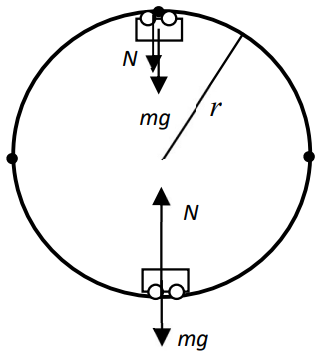
\includegraphics[scale=.5]{assets/rollercoaster.png}
	\caption{Rollercoaster on vertical circular track}
\end{marginfigure}
\begin{example}{}{rollercoaster}
	A rollercoaster of mass \(m\) moves along a vertical circular track of radius \(r\).
	At the top of the track, both \(mg\) and \(N_\text{top}\) act downwards to provide the centripetal acceleration.
	\[ma_c = N_\text{top} + mg\]
	At the top of the track, the minimum speed \(v_\text{min}\) occurs when \(N_\text{top}=0\).
	\[v_\text{min} = \sqrt{rg}\]

	At the bottom of the track, \(mg\) still acts downwards, but \(N_\text{bottom}\) acts upwards.
	\[ma_c = N_\text{bottom} - mg\]
\end{example}
